Este experimento busca validar las condiciones necesarias que debe tener una secuencia de entrada para que el algoritmo \texttt{LDC} pueda optimizar al momento de ser construido para una predicción \emph{online}, dado esto utilizaremos sesiones largas que entreguen redundancia en los accesos que permita al modelo de navegación ser más comprimido sin perder una métrica considerable para funcionar, según lo anterior realizamos las siguientes iteraciones con las particiones de data que cumplen: 
	
	\begin{figure}[h] 
		\centering
		\resizebox{.7\textwidth}{!}{
		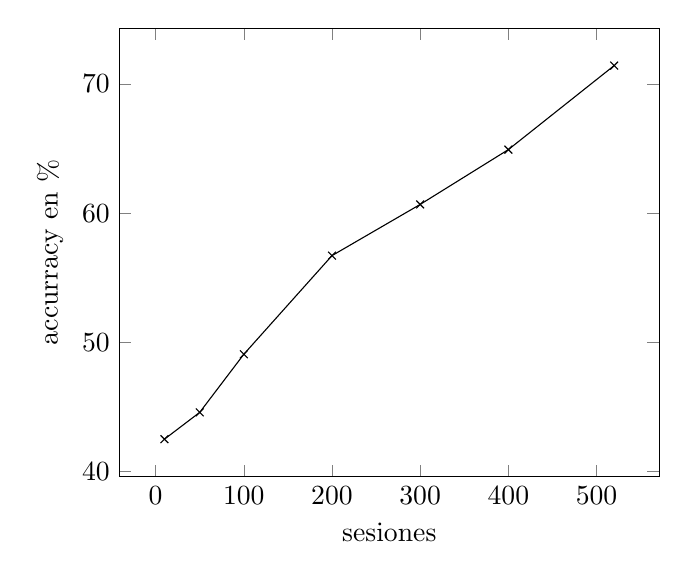
\begin{tikzpicture}
		\begin{axis}[
			xlabel= sesiones,
			ylabel=accurracy en \% ]
		\addplot[color=black,mark=x] coordinates {
			(10 ,  42.5190839694656 )
			(50 ,  44.595041322314 )
	 		(100 , 49.089861751152 )
	 		(200 , 56.7230538922155 )
	 		(300 , 60.6837606837608 )
	 		(400 , 64.9253731343282 )
	 		(520 , 71.4285714285715 )			
		};
		\end{axis}
		\end{tikzpicture}
		}
		\caption{Gráfico de Accuracy para sesiones mayores de 100 símbolos}
		\label{fig:sim}
	\end{figure}
	
	
	Sean la sesiones de entrenamiento de tamaño $T$, con un valor  $T(100) = 49 \% $ sobre un set de evaluación $E(100) = 900 \mbox{ sesiones}$ , nuestro modelo propuesto al igual que en el experimento \ref{exp1}, entrega un punto mínimo el cual al menos da un $50\%$ de acierto sobre el total de $535$ sesiones de usuarios, con una secuencia mínima de $100$ símbolos. Planteado de otra forma, sólo con el $20\%$ del total de datos de entrenamiento nuestro motor de predicción ya alcanza un \emph{Accurracy} que es mucho mejor que un predictor aleatorio sobre el alfabeto del experimento. Siendo este valor bastante optimista acorde a los puntos óptimos del predictor que use la menor cantidad de recursos.
	
	
	\begin{figure}[h] \label{fig:sim}
	\centering
		\resizebox{.7\textwidth}{!}{
		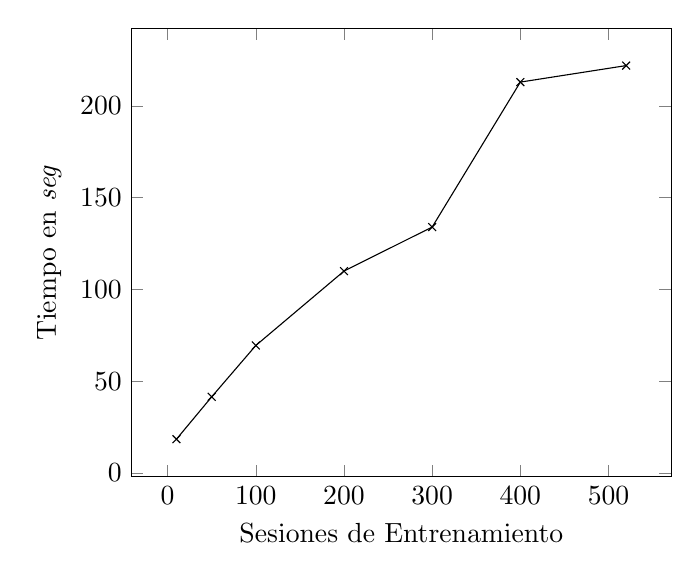
\begin{tikzpicture}
		\begin{axis}[
		xlabel= Sesiones de Entrenamiento ,
		ylabel=Tiempo en \emph{seg} ]
		\addplot[color=black,mark=x] coordinates {
			(10 ,  18.4)
			(50 ,  41.5)
			(100 , 69.46)
			(200 , 110)
			(300 , 134)
			(400 , 213)
			(520 , 222)	
		};
		\end{axis}
		\end{tikzpicture}
		}
		\caption{Gráfico de tiempo vs sesiones de entrenamiento\\ para sesiones mayores de 100 símbolos}
		
	\end{figure}


\begin{table}[h]
	\centering
	\caption{Tabla resumen experimento 4}
	\label{my-label}
	\begin{tabular}{ccccc}
		\textbf{pruebas} & \textbf{entrenamiento} & \textbf{accuracy} & \textbf{nodos} & \textbf{niveles} \\
		990              & 10                     & 0,21422649140546  & 38             & 5                \\
		950              & 50                     & 0,3104531085353   & 95             & 5                \\
		900              & 100                    & 0,393259176863181 & 132            & 5                \\
		800              & 200                    & 0,418698372966207 & 181            & 5                \\
		700              & 300                    & 0,421454458750596 & 208            & 5                \\
		600              & 400                    & 0,426323038397328 & 241            & 5                \\
		500              & 500                    & 0,419799599198396 & 264            & 5                \\
		400              & 600                    & 0,453634085213033 & 288            & 5                \\
		300              & 700                    & 0,407892976588628 & 308            & 5                \\
		200              & 800                    & 0,439736180904522 & 326            & 5                \\
		100              & 900                    & 0,429539842873176 & 349            & 5               
	\end{tabular}
\end{table}

\begin{table}[]
	\centering

	\label{my-label}
	\resizebox{0.9\textwidth}{!}{
	\begin{tabular}{lccccccccccccccccc}
		\textbf{símbolo}    & A    & B    & C   & D   & E   & F   & G   & H    & I   & J   & K   & L   & M   & N   & O   & P  & Q  \\
		\textbf{frecuencia} & 2162 & 1044 & 269 & 757 & 225 & 815 & 681 & 1207 & 370 & 278 & 233 & 453 & 502 & 860 & 102 & 10 & 32
	\end{tabular}
	}
	\caption{Tabla resumen de simbolos y frecuencia para experimento 4}
\end{table}

	Congruente con lo anterior podemos ver que sin tener un margen de error superior a la porción de datos seleccionado logramos un latencia de consulta predictiva en línea de alrededor de 70 \emph{seg}, el cual para ser implementado y consumido como ya se había mencionado antes como un algoritmo predictivo como servicio \emph{REST}, esta dentro del promedio aceptable.

	\begin{figure}[h] 
		\centering
		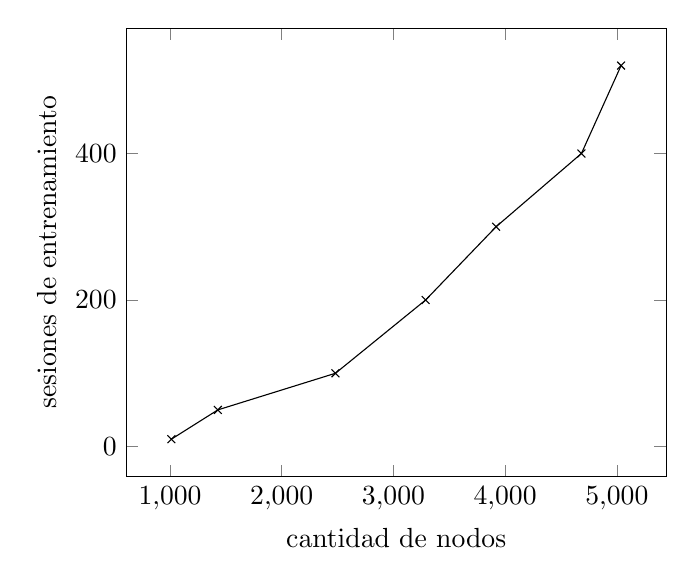
\begin{tikzpicture}
		\begin{axis}[
			xlabel= cantidad de nodos,
			ylabel= sesiones de entrenamiento  ]
		\addplot[color=black,mark=x] coordinates {
			(1012,10 )
			(1428,50 )
			(2481,100 )
			(3288,200 )
			(3919,300 )
			(4683,400 )
			(5038,520 )	
		};
		\end{axis}
		\end{tikzpicture}	
		\caption{Gráfico de cantidad de nodos vs sesiones de entrenamiento para sesiones mayores de 100 símbolos}
	  \label{fig:sim}
	\end{figure}


	Otro de los puntos  considerado aceptable, es que dado un set de entrenamiento $T(100)$, solo necesitaremos menos de la mitad de nodos que se requieren para llegar a un valor de predicción bueno, a diferencia de una partición de entrenamiento que requiere más del $90\%$ de nodos del total del set de datos.\\
	

	
	\begin{figure}[h] 
		\centering
			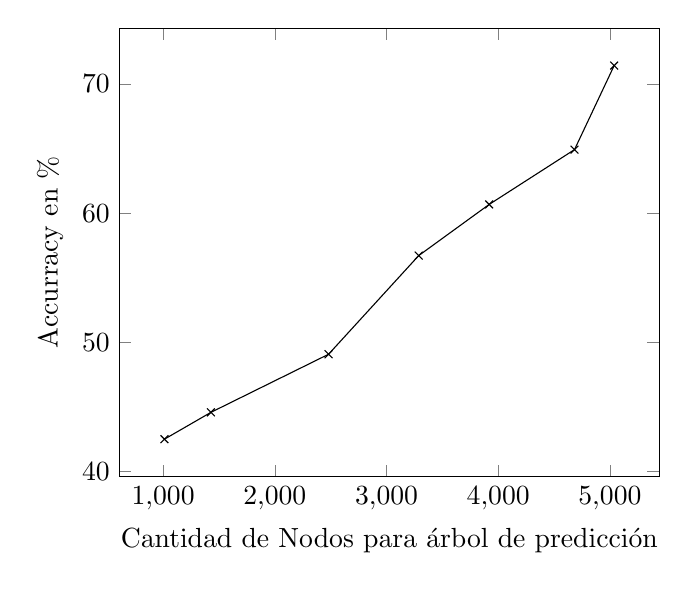
\begin{tikzpicture}
			\begin{axis}[
			xlabel=Cantidad de Nodos para árbol de predicción,
			ylabel=Accurracy en \%  ]
			\addplot[color=black,mark=x] coordinates {
				(1012,42.5190839694656 )
				(1428,44.595041322314 )
				(2481,49.089861751152 )
				(3288,56.7230538922155 )
				(3919,60.6837606837608 )
				(4683,64.9253731343282 )
				(5038,71.4285714285715 )	
			};	
			\end{axis}
			\end{tikzpicture}	
			\caption{Gráfico de cantidad de nodos vs Accuracy para sesiones mayor de 100 símbolos}
		\label{fig:sim}
	\end{figure}



	Finalmente podemos señalar que la tasa de \emph{Accuracy}, aún  subiendo al doble la cantidad de nodos para construir un \emph{trie} de \texttt{LZ78}, con mayor información  para predecir alcanza un rendimiento aceptable respecto de la compresión realizada. De todas maneras también se cumple que la cantidad de nodos del entrenamiento es directamente proporcional a la métrica seleccionada.